%
% main.tex -- Paper zum Thema <zeta>
%
% (c) 2020 Autor, OST Ostschweizer Fachhochschule
%
% !TEX root = ../../buch.tex
% !TEX encoding = UTF-8
%
\chapter{Die Summe aller natürlichen Zahlen und die riemannsche Zeta-Funktion\label{chapter:zeta}}
\kopflinks{Die Summe aller natürlichen Zahlen und die riemannsche Zeta-Funktion}
\begin{refsection}
\chapterauthor{Melissa Haumüller}

\input{papers/zeta/teil0_einleitung.tex}
\input{papers/zeta/teil1_konvergenz_divergenz.tex}
%
% teil2.tex -- Beispiel-File für teil2 
%
% (c) 2020 Prof Dr Andreas Müller, Hochschule Rapperswil
%
% !TEX root = ../../buch.tex
% !TEX encoding = UTF-8
%
\section{Riemannsche Zeta-Funktion}\label{Riemannsche Zeta-Funktion}
\kopfrechts{Riemannsche Zeta-Funktion}

Die riemannsche Zeta-Funktion wurde 1859 von Bernhard Riemann untersucht und ist eine zentrale Funktion der
\index{Bernhard Riemann}%
\index{Riemann, Bernhard}%
analytischen Zahlentheorie. Sie wird üblicherweise als unendliche Reihe
\index{analytische Zahlentheorie}%
definiert. Für alle komplexen Variablen $s$ mit Realteil grösser als 1 ergibt sich ihre Darstellung als
\[
\zeta(s) = \sum_{n = 1}^{\infty}\frac{1}{n^{s}}.
\]
Diese Definition beschreibt eine Dirichlet-Reihe, deren Konvergenz für $\operatorname{Re}(s) > 1$ gewährleistet ist. 
Bereits in diesem Definitionsbereich zeigt die Funktion bemerkenswerte Eigenschaften. 
So nimmt sie für bestimmte Argumente konkrete Werte an, wie in Tabelle \ref{tab:zeta} dargestellt ist.

%
% table.tex -- Tabelle der Zeta-Werte
%
% (c) 2026 Prof Dr Andreas Müller
%
\begin{table}
\centering
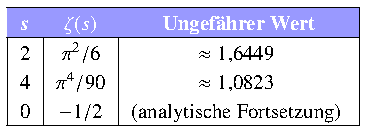
\includegraphics{papers/zeta/images/tabular.pdf}
\caption{Ausgewählte Werte der Zeta-Funktion}
\label{tab:zeta}
\end{table}


Besonders bemerkenswert ist hier der Wert $\zeta$(2) = $\frac{\pi^2}{6}$, den Euler bereits 1735 nachwies, bekannt als das Basler Problem (siehe Kapitel \ref{chapter:basel}).
\index{Euler, Leonhard}%
\index{Basel-Problem}%
Die letze Zeile der Tabelle gehört jedoch nicht zum ursprünglichen Definitionsbereich (s > 1), sondern ist nur durch analytische Fortsetzung erreichbar. 

Bereits der Fall $s = 0$ zeigt, dass es sich bei solchen divergenten Werten nicht um Einzelfälle handelt.
Setzt man $s = 0$ formal in die Reihendefinition ein, so erhält man
\[
\zeta(0) \overset{?}{=} \sum_{n=1}^{\infty} 1 = 1 + 1 + 1 + \ldots,
\]
also genau die in Abschnitt~\ref{konvergente-und-divergente-reihen} als bestimmt divergent identifizierte Reihe.
Dennoch liefert die analytische Fortsetzung dafür den wohldefinierten Wert $\zeta(0) = -1/2$ (vgl. Tabelle~\ref{tab:zeta}).
Das deutet darauf hin, dass hinter solchen Werten eine globale, einheitliche Methode steht und nicht eine Sammlung von Einzelfällen, die man je einzeln erklären müsste.

Ein besonders interessanter Fall ist $s = -1$, mit dem wir uns im weiteren Verlauf dieses Papers eingehender beschäftigen.
Setzt man diesen Wert formal in die Reihendefinition ein, so erhält man
\[
\zeta(-1) \overset{?}{=} \sum_{n=1}^{\infty} \frac{1}{n^{-1}} = \sum_{n=1}^{\infty} n = 1 + 2 + 3 + \ldots,
\]
also genau die Summe aller natürlichen Zahlen.
Dieses Einsetzen ist jedoch nicht zulässig: Die Reihe $\sum_{n=1}^{\infty} n^{-s}$ konvergiert nur für $\operatorname{Re}(s) > 1$, für $s = -1$ ist sie schlicht divergent und die Reihendefinition liefert keinen Wert.
Der Wert von $\zeta(-1)$ kann also nicht direkt aus der Reihe berechnet werden, sondern muss auf anderem Weg gewonnen werden.
Wie dies mit Hilfe der analytischen Fortsetzung gelingt, wird in Abschnitt~\ref{Analytische Fortsetzung} gezeigt.

\begin{figure}
	\centering
	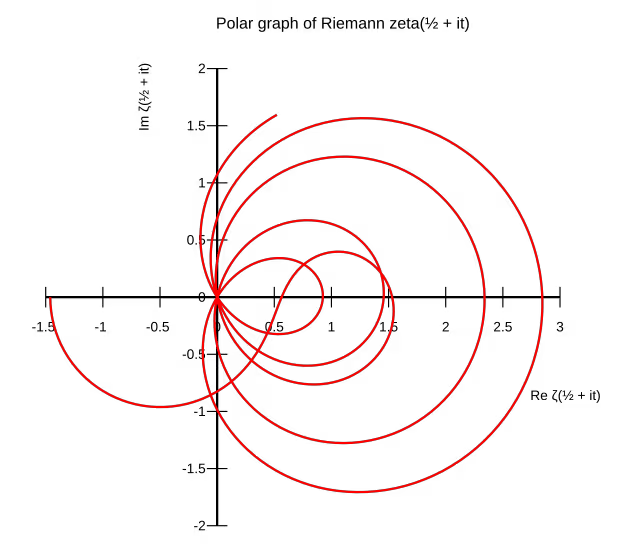
\includegraphics[width=1.0\linewidth]{papers/zeta/Abbildung_Zeta.png}
	\caption{Werte der riemannschen Zeta-Funktion auf der kritischen Geraden $\operatorname{Re}(s) = \frac{1}{2}$, dargestellt als Polarkurve $\zeta\bigl(\frac12 + it\bigr)$ für variierendes $t$.}
	\label{fig:abbildungzeta}
\end{figure}

Die spiralförmige Darstellung in Abbildung \ref{fig:abbildungzeta} zeigt die Werte der Zeta-Funktion $\zeta(s)$ auf der kritischen Geraden $\operatorname{Re}(s) = \frac{1}{2}$, das heisst für $s = \frac12 + it$ mit variierendem reellen Parameter $t$. Die Schnittpunkte der Kurve mit dem Ursprung (sichtbar als die Stellen, an denen die Spirale durch den Mittelpunkt verläuft) entsprechen den sogenannten nicht-trivialen Nullstellen der Zeta-Funktion, die auf dieser Geraden liegen. Dass tatsächlich alle nicht-trivialen Nullstellen auf der Linie $\operatorname{Re}(s) = \frac{1}{2}$ liegen, ist Gegenstand der berühmten, bis heute unbewiesenen riemannschen Vermutung, einem der bedeutendsten offenen Probleme der Mathematik.
\index{kritische Gerade}%

Nützlich ist die riemannsche Zeta-Funktion ebenfalls, um eine Annäherung der Primzahlfunktion zu schaffen. 
Das Euler-Produkt
\[
\zeta(s) = \prod_{p \ \text{prim}} \frac{1}{1 - p^{-s}}
\]
beschreibt eine geometrische Reihe, welche den Zusammenhang aller Primzahlen aufzeigt. 

\begin{figure}
	\centering
	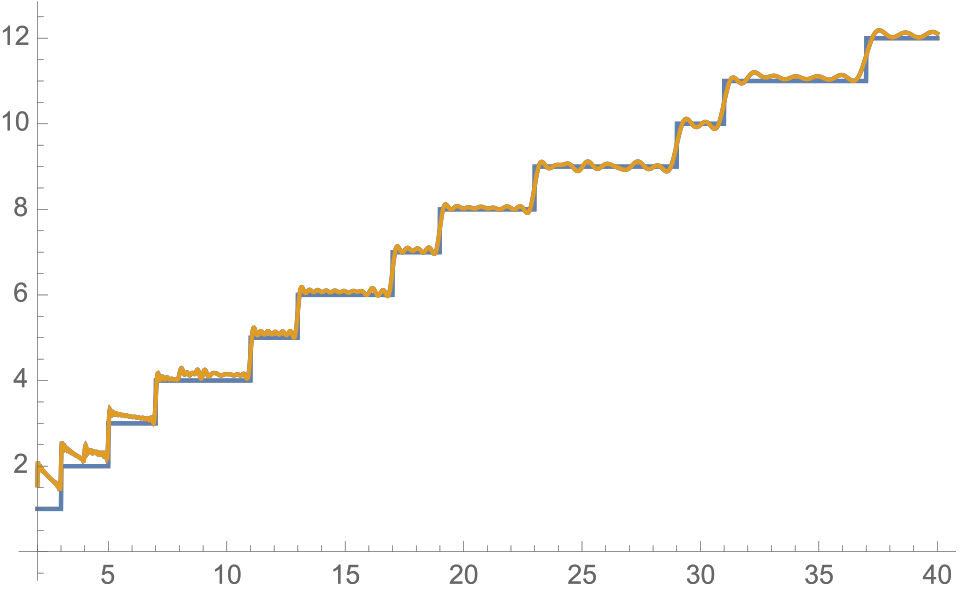
\includegraphics[width=0.7\linewidth]{papers/zeta/Primzahlen.png}
	\caption{Primzahlzählfunktion}
	\label{fig:primzahlen}
\end{figure}

Die blaue Treppenkurve in Abbildung~\ref{fig:primzahlen} zeigt die Primzahlzählfunktion $\pi(x)$, welche für jede reelle Zahl $x$ angibt, wie viele Primzahlen kleiner oder gleich $x$ existieren.
\index{Primzahlzählfunktion}%
Die orangefarbene Kurve stellt den logarithmischen Integralausdruck $\operatorname{Li}(x)$ dar, eine glatte, sprungfreie Funktion. Er wird in Definition \ref{buch:intalg:risch:def:integrallogarithmus} eingeführt.
Das ist eine von Riemann entwickelte Näherungsformel für $\pi(x)$, die direkt aus der Zeta-Funktion abgeleitet wird. Eine ausführliche, gut nachvollziehbare Herleitung deses Zusammenhangs findet sich bei \cite{edwards1974riemann}.
Man erkennt, wie eng beide Kurven beieinander liegen: $\operatorname{Li}(x)$ approximiert die Verteilung der Primzahlen, wobei die relative Genauigkeit dieser Näherung mit wachsendem $x$ zunimmt.


%
% teil3.tex -- Beispiel-File für Teil 3
%
% (c) 2020 Prof Dr Andreas Müller, Hochschule Rapperswil
%
% !TEX root = ../../buch.tex
% !TEX encoding = UTF-8
%
\section{Analytische Fortsetzung
\label{Analytische Fortsetzung}}
\kopfrechts{Analytische Fortsetzung}

Die analytische Fortsetzung ist ein Konzept aus der komplexen Analysis, mit dem eine holomorphe Funktion über ihren ursprünglichen Definitionsbereich hinaus erweitert werden kann.
Eine ausführliche Einführung dazu findet sich in Abschnitt 5.3 des Buches.
Grundsätzlich wird dabei eine neue Funktion konstruiert, die auf dem ursprünglichen Definitionsbereich mit der alten Funktion übereinstimmt, aber auch ausserhalb davon definiert ist.

In der Anwendung auf die riemannsche Zeta-Funktion kann eine solche analytische Fortsetzung fast auf die gesamte komplexe Ebene angewendet werden.
\index{analytische Fortsetzung}%
Die einzige Ausnahme ist der Punkt bei $s = 1$.
%Beschreiben anhand Bild wie so eine Funktion erweitert wird anhand prinzip dass man definitionsbereich von Funktionen sucht, die in einem gewissen Bereich sich überschneiden

\subsection{Anwendung auf die Zeta-Funktion\label{Anwendung auf die Zeta-Funktion}}

Wie bereits in Abschnitt~\ref{Riemannsche Zeta-Funktion} erwähnt, ist die Reihendarstellung
\index{zeta-Funktion@$\zeta$-Funktion!Reihendarstellung}%
\[
\zeta(s) = 1 + \frac{1}{2^{s}} + \frac{1}{3^{s}} + \frac{1}{4^{s}} + \ldots
\]
nur für $\operatorname{Re}(s) > 1$ korrekt.

Wie in Kapitel \ref{chapter:hankel} hergeleitet wird, liefert die analytische Fortsetzung für die Zeta-funktion die sogenannte Funktionalgleichung, welche $\zeta(s)$ mit $\zeta(1-s)$ verbindet:
\index{Funktionalgleichung}%
\[
\zeta(s) = 2^s \pi^{s-1} \sin\left(\frac{\pi s}{2}\right) \Gamma(1 - s)\,\zeta(1 - s).
\]
Die Gamma-Funktion $\Gamma$, die in dieser Formel auftritt, wird in Kapitel \ref{chapter:gamma} eingeführt.
\index{Gamma-Funktion@$\Gamma$-Funktion}%
Die Funktionalgleichung gilt für (fast) alle $s \in \mathbb{C}$ und liefert damit auch für negative $s$ einen wohldefinierten Wert von $\zeta(s)$, obwohl die ursprüngliche Reihe dort gar nicht konvergiert.

Setzt man $s = -1$ ein, so verbindet die Funktionalgleichung $\zeta(-1)$ mit $\zeta(2)$:
\[
\zeta(-1) = 2^{-1} \pi^{-2} \sin\left(-\frac{\pi}{2}\right)\Gamma(2)\,\zeta(2).
\]
Der Wert $\zeta(2)$ ist uns bereits bekannt: Es handelt sich, wie in Abschnitt~\ref{Riemannsche Zeta-Funktion} erwähnt, um das Basler Problem, welches Euler 1735 löste, mit dem Resultat $\zeta(2) = \pi^2/6$.
\index{Basel-Problem}%
\index{Euler, Leonhard}%

Mit
\[
\sin\left(-\frac{\pi}{2}\right) = -1, \quad \Gamma(2) = 1! = 1, \quad \zeta(2) = \frac{\pi^2}{6}
\]
folgt
\[
\zeta(-1) = \frac{1}{2} \cdot \frac{1}{\pi^2} \cdot (-1) \cdot 1 \cdot \frac{\pi^2}{6} = -\frac{1}{12}.
\]
Damit ist gezeigt, dass sich der Wert $-\frac{1}{12}$ nicht aus der divergenten Reihe selbst ergibt, sondern aus der Funktionalgleichung, die die analytische Fortsetzung der Zeta-Funktion liefert.





\input{papers/zeta/teil4_fazit.tex}

\printbibliography[heading=subbibliography]
\end{refsection}
